% !TEX program = pdflatex
%
% =====================================================================
%  SG-AMP: Stability-Gated Adversarial Motion Priors with
%  Phase-Conditioned Discriminator for Natural and Robust Bipedal Locomotion
%
%  IEEE CONFERENCE TEMPLATE VERSION (IEEEtran, two-column), 6-page.
%  Compile with:  pdflatex + bibtex + pdflatex x2
%    pdflatex sgamp_paper_IEEE
%    bibtex   sgamp_paper_IEEE
%    pdflatex sgamp_paper_IEEE
%    pdflatex sgamp_paper_IEEE
% =====================================================================

\documentclass[conference]{IEEEtran}
% \IEEEoverridecommandlockouts % uncomment only if you add a funding \thanks{} in \title
\usepackage{amsmath,amssymb,amsfonts}
\usepackage{graphicx}
\usepackage{booktabs}
\usepackage{textcomp}
\usepackage{float}
% The `algorithm` + `algpseudocode` bundles are not installed in this MiKTeX
% setup, so we declare a minimal "Algorithm" float via the `float` package and
% typeset the pseudocode manually (single column).
\newfloat{algorithm}{tbp}{loa}
\floatname{algorithm}{Algorithm}
% Tighten float spacing to remove blank gaps between figure captions and text
\setlength{\textfloatsep}{11pt plus 2pt minus 2pt}
\setlength{\dbltextfloatsep}{11pt plus 2pt minus 2pt}
\setlength{\abovecaptionskip}{7pt plus 2pt minus 2pt}
\setlength{\belowcaptionskip}{7pt plus 2pt minus 2pt}
% Allow only one full-width float per page top, so the wide comparison table
% goes to the experiments page instead of stacking underneath Fig. 1.
\setcounter{dbltopnumber}{1}

\begin{document}

\title{Stability-Gated Adversarial Motion Priors with Phase-Conditioned Discriminator for Natural and Robust Bipedal Locomotion%
}

% ---- Author block: 4 authors, IEEE conference format (ordinal name style) ----
% Affiliation 1: College of Robotics, Beijing Union University, Beijing, China
% Affiliation 2: Beijing Zoyi Technology Co., Ltd., Beijing, China
\author{\IEEEauthorblockN{1\textsuperscript{st} Jiahong Li}
\IEEEauthorblockA{\textit{College of Robotics} \\
\textit{Beijing Union University}\\
Beijing, China \\
lijiahong.bit@gmail.com}
\and
\IEEEauthorblockN{2\textsuperscript{nd} Xuepeng Dong}
\IEEEauthorblockA{\textit{College of Robotics} \\
\textit{Beijing Union University}\\
Beijing, China \\
dongxuepeng7@gmail.com}
\and
\IEEEauthorblockN{3\textsuperscript{rd} Shengli Xu}
\IEEEauthorblockA{\textit{Beijing Zoyi Technology Co., Ltd.}\\
Beijing, China \\
dr.xu@zoyitech.com}
\and
\IEEEauthorblockN{4\textsuperscript{th} Beiyan Jiang*}
\IEEEauthorblockA{\textit{College of Robotics} \\
\textit{Beijing Union University}\\
Beijing, China \\
jqrbeiyan@buu.edu.cn}
*Corresponding author}

\maketitle

\begin{abstract}
Endowing bipedal robots with natural yet robust gaits is a central challenge. Adversarial Motion Priors (AMP) distill motion-capture style into a policy, but vanilla AMP has three limitations: a physics-blind style reward, a phase-agnostic discriminator that induces within-cycle jitter, and a fixed task--style weight that conflicts on difficult terrain. We propose \emph{Stability-Gated Adversarial Motion Priors} (SG-AMP) with three lightweight modules: (i) a Center-of-Pressure (CoP) stability margin gates the style reward through a smooth sigmoid, grounding style in physics; (ii) a foot-contact-driven gait phase is injected into the discriminator for phase-consistent learning; and (iii) the style weight follows an exponential moving average of the stability margin, forming a self-paced curriculum. Using only foot contact forces and foot-sole geometry from the physics backend (Isaac Sim PhysX / MuJoCo), SG-AMP raises external-push and rough-terrain survival to 0.736 and 0.486 (+59.3\% and +122.9\% over AMP) and cuts spectral energy by 63.5\%, with ablations verifying each module.
\end{abstract}

\begin{IEEEkeywords}
Bipedal locomotion; Adversarial motion priors; Reinforcement learning; Center of pressure; Gait phase; Stability
\end{IEEEkeywords}

\section{Introduction}
\label{sec:introduction}

Reinforcement learning (RL) has produced robust legged locomotion, from agile quadrupedal skills \cite{hwangbo2019anymal}, challenging-terrain traversal \cite{lee2020challenging}, and rapid adaptation \cite{kumar2021rma}, to bipedal/humanoid locomotion from proprioceptive blind walking \cite{singh2022footsteps}, perceptive locomotion over irregular terrain \cite{vanmarum2023perceptive, song2025gaitadaptive}, and general policies over challenging terrain \cite{radosavovic2024challenging, huang2026coremoe}. Recent humanoid controllers now transfer zero-shot to real hardware \cite{radosavovic2024real} and enable whole-body imitation, teleoperation, and unified multi-mode control \cite{cheng2024exbody, he2024hover, fu2024humanplus, he2024omnih2o}. Yet the resulting gaits are often stiff, bent-kneed, and lack biological fluidity \cite{zhang2025gmp}, because hand-crafted task rewards cannot capture the subtle balance and coordination of human gait \cite{peng2021amp}.

Adversarial Motion Priors (AMP) \cite{peng2021amp} distill motion-capture (MoCap) style into a policy via a discriminator, and remain the dominant route to naturalness \cite{zhang2025gmp, guo2026tgmp}. The AMP lineage has since scaled into reusable skill embeddings (ASE) \cite{peng2022ase}, conditional latent models (CALM) \cite{tessler2023calm}, and universal motion representations (PULSE) \cite{luo2024pulse}, yielding increasingly fluid and controllable motion. However, vanilla AMP has three well-documented limitations \cite{zhang2025gmp, guo2026tgmp}: (i) the discriminator yields a physics-blind style reward carrying no stability information, so style can reward unstable motion; (ii) the prior is phase-agnostic, so the style reward fluctuates within a gait cycle and induces high-frequency jitter; and (iii) the fixed task--style weight creates an objective conflict on difficult terrain, where stability and style compete.

We propose \emph{Stability-Gated Adversarial Motion Priors} (SG-AMP), which inserts an automatic physics valve---the Center of Pressure (CoP)---between the discriminator's style signal and the policy's stability objective, while making the discriminator phase-aware and the style injection self-paced. Our contributions are three independently ablating modules: (1) a \emph{CoP-gated style reward} that gates the style reward by a sigmoid of the CoP stability margin, grounding style in physics; (2) a \emph{phase-conditioned discriminator} that injects a foot-contact-driven gait phase $(\cos\phi_t,\sin\phi_t)$ for phase-consistent learning; and (3) a \emph{stability-driven adaptive style-weight curriculum} $\lambda_t=\lambda_{\max}\bar g_t$ that resolves the style--stability conflict without manual tuning. Unlike CoP used as a quadruped \emph{task reward} \cite{hwang2026footposition} or the task-side Foothold Penalty of T-GMP \cite{guo2026tgmp}, we are the first to use CoP stability as a \emph{gate on the AMP style reward}. The method requires only foot contact forces and foot-sole geometry, available from the physics backend (Isaac Sim PhysX for training, MuJoCo for sim2sim), so we study it purely in simulation on a self-developed biped.

\section{Related Work}
\label{sec:related_work}

Following generative adversarial imitation learning \cite{ho2016gail} and reference-motion imitation \cite{peng2018deepmimic}, AMP \cite{peng2021amp} brings GANs to stylized control: a discriminator scores state transitions and a style reward steers the policy to imitate reference motion; for humanoids, retargeted MoCap is treated as real and policy transitions as fake \cite{zhang2025gmp, guo2026tgmp}. Because the style reward is an ambiguous scalar and adversarial training is unstable, GMP \cite{zhang2025gmp} replaces the discriminator with a frozen conditional VAE for dense joint/keypoint supervision, and T-GMP \cite{guo2026tgmp} conditions this latent manifold on terrain and adds a Foothold Penalty. In contrast, we keep the discriminator and only modify its input (phase, contribution 2) and output usage (CoP gating, contribution 1) at lower implementation cost.

For multi-terrain humanoid control, contrastive mixture-of-experts methods \cite{ma2026cmoe, huang2026coremoe}, model-assisted RL \cite{crismariu2026march}, and skill-graph switching \cite{lau2026switch} organize skills and terrains orthogonally to our focus on the style quality and stability of a single gait. CoP-based stability is a classical criterion rooted in zero-moment point (ZMP) theory \cite{vukobratovic2004zmp, kajita2003zmp}: Hwang et al.~\cite{hwang2026footposition} use $\min d(p_{\mathrm{CoP}},\text{edges})$ as a quadruped \emph{task reward}. We instead use it as a \emph{gate on the style reward}, so naturalness and stability cooperate rather than compete. Phase-based periodic rewards have been used to learn common gaits \cite{siekmann2021periodic}; we inject phase into the AMP \emph{discriminator} as a structural prior rather than a task reward.

\section{Method}
\label{sec:method}

\subsection{Problem Formulation and AMP Background}
\label{subsec:method_prelim}

We model locomotion as a Markov decision process $(\mathcal{S},\mathcal{A},T,r,\gamma)$, where the observation $s_t$ is proprioception (base orientation/angular velocity, joint positions/velocities, previous action) and the action $a_t$ is the joint-level PD target. The policy $\pi_\theta$ is trained with PPO \cite{schulman2017ppo}---a first-order trust-region method \cite{schulman2015trpo}---in Isaac Sim (PhysX backend) and cross-validated in MuJoCo \cite{todorov2012mujoco}. Given reference transitions $\mathcal{M}=\{(s,s')\}$ (MoCap-retargeted or expert-generated), vanilla AMP trains a discriminator $D_\psi$ to distinguish reference (real) from policy (fake) transitions:
\begin{multline}
\mathcal{L}_D = \tfrac{1}{2}\,\mathbb{E}_{(s,s')\sim\mathcal{M}}\big[(D_\psi(s,s')-1)^2\big]
\\
+ \tfrac{1}{2}\,\mathbb{E}_{(s,s')\sim\pi_\theta}\big[(D_\psi(s,s')+1)^2\big],
\label{eq:amp_disc}
\end{multline}
and provides the style reward
\begin{equation}
r^{\mathrm{style}}_t = \max\big(0,\,1-\tfrac{1}{4}(D_\psi(s_t,s_{t+1})-1)^2\big),
\label{eq:amp_style}
\end{equation}
so the policy is trained with $r_t = r^{\mathrm{task}}_t + w^{\mathrm{style}} r^{\mathrm{style}}_t$, where $r^{\mathrm{task}}_t$ collects task rewards and $w^{\mathrm{style}}$ is a fixed weight. We apply three lightweight modifications on top of \eqref{eq:amp_disc}--\eqref{eq:amp_style}, summarized in Fig.~\ref{fig:overview}.

\begin{figure*}[t]
  \centering
  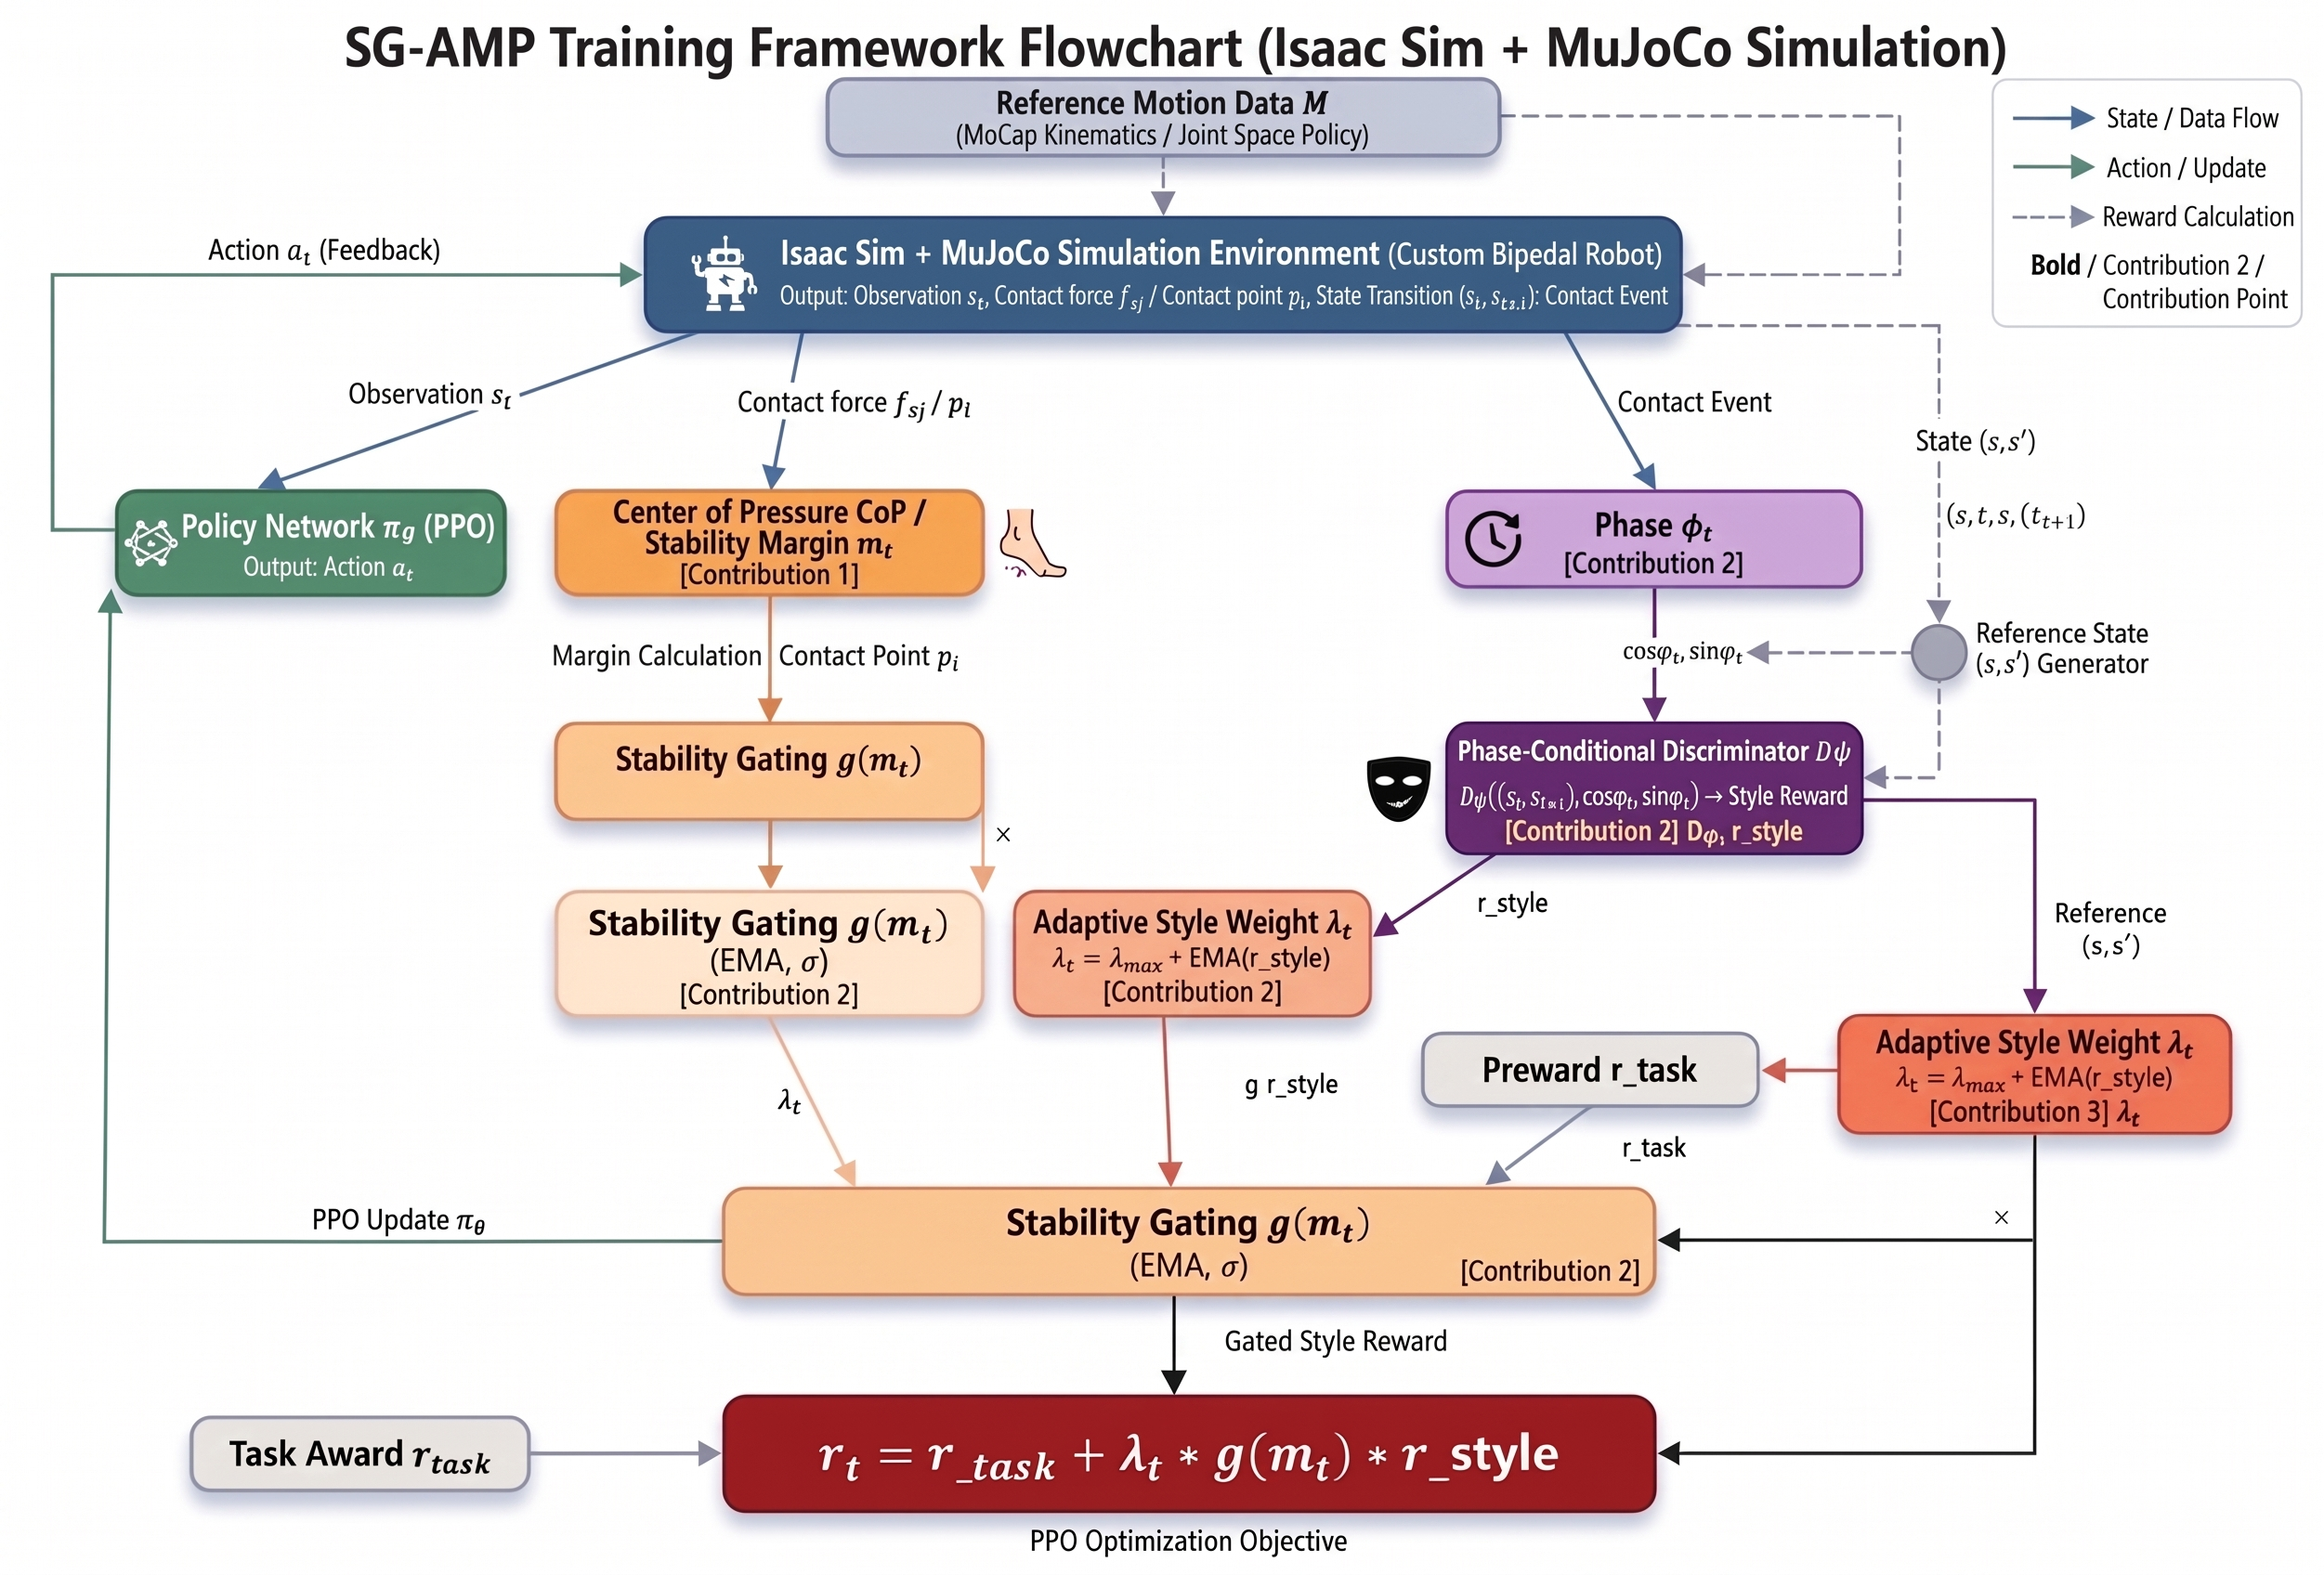
\includegraphics[width=0.85\linewidth]{fig1.jpg}
  \caption{Overview of SG-AMP. Three lightweight modifications are made on top of vanilla AMP: (1) the style reward is gated by the CoP-based stability margin $g(m_t)$; (2) the discriminator is conditioned on the gait phase $(\cos\phi_t,\sin\phi_t)$; and (3) the style weight $\lambda_t=\lambda_{\max}\cdot\bar g_t$ follows an EMA of the gate. All signals are available from the physics backend (Isaac Sim PhysX for training, MuJoCo for sim2sim).}
  \label{fig:overview}
\end{figure*}

\subsection{CoP-Gated Style Reward}
\label{subsec:method_cop}

Let $\mathcal{C}=\{i\mid f_{z,i}>f_{\mathrm{th}}\}$ denote the feet in active contact ($f_{\mathrm{th}}=1$\,N), and $p_{i,k},f_{z,i,k}$ the position and vertical force of the $k$-th contact element on foot $i$ (a $3\times2$ grid, $K=6$). The global Center of Pressure (CoP) is
\begin{equation}
p_{\mathrm{CoP}} = \frac{\sum_{i\in\mathcal{C}} \sum_{k=1}^K f_{z,i,k}\, p_{i,k}}{\sum_{i\in\mathcal{C}} \sum_{k=1}^K f_{z,i,k}}.
\label{eq:cop}
\end{equation}
Projecting onto the ground plane, the support polygon $\mathcal{S}_t$ is the convex hull of the active foot contact vertices, and the dynamic stability margin is the minimum signed distance from the CoP to the polygon edges:
\begin{equation}
m_t = \min_{e\in\partial\mathcal{S}_t}\ d_{\mathrm{signed}}\big(p_{\mathrm{CoP}},\,e\big),
\label{eq:margin}
\end{equation}
positive when the CoP lies inside $\mathcal{S}_t$ and negative outside. When the robot tilts or lands on an edge, contact force concentrates on outer elements and drives $p_{\mathrm{CoP}}$ toward or beyond the boundary ($m_t\le0$). We gate the style reward with a smooth sigmoid (Fig.~\ref{fig:cop}):
\begin{equation}
g(m_t) = \sigma\!\left(\frac{m_t - m_0}{\kappa}\right),\qquad
r^{\mathrm{style}}_t = g(m_t)\cdot r^{\mathrm{amp}}_t,
\label{eq:gate}
\end{equation}
with $m_0=0.025$\,m and $\kappa=0.006$\,m. When $m_t\gg m_0$ the gate is $\approx1$ (full style); when $m_t\le0$ the gate $\to0$, attenuating style and prioritizing recovery. The gate is a post-hoc multiplication on the scalar style reward, so it adds no gradient path and is robot-agnostic.

\begin{figure}[t]
  \centering
  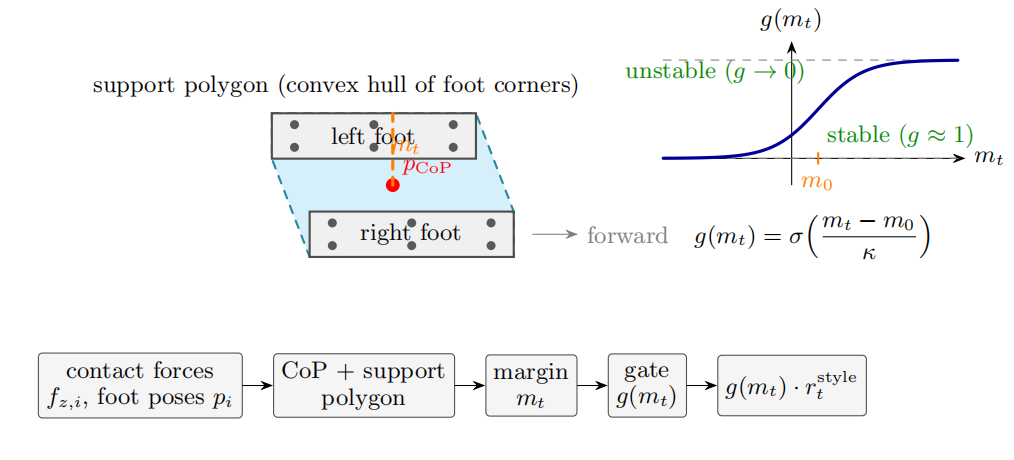
\includegraphics[width=\linewidth]{fig2.jpg}
  \caption{CoP-gated style reward (contribution 1). The CoP is computed from contact forces, and the minimum signed distance $m_t$ to the support-polygon edges defines a dynamic stability margin. The smooth gate $g(m_t)=\sigma((m_t-m_0)/\kappa)$ scales the AMP style reward so style supervision is active only when the robot is dynamically stable.}
  \label{fig:cop}
\end{figure}

\subsection{Phase-Conditioned Discriminator}
\label{subsec:method_phase}

Bipedal gait is strongly periodic; a phase-agnostic discriminator makes the style reward fluctuate within a cycle and induces jitter. We maintain a gait phase $\phi_t\in[0,2\pi)$ driven by foot-contact events: advance a clock $\phi_{t+\Delta t}=\phi_t+2\pi f_{\mathrm{cmd}}\Delta t$, and align/reset it at heel strikes. We encode $(\cos\phi_t,\sin\phi_t)$ and inject it into the discriminator (Fig.~\ref{fig:phase}):
\begin{equation}
D_\psi\big(s_t,s_{t+1},\cos\phi_t,\sin\phi_t\big).
\label{eq:phase_disc}
\end{equation}
The reference dataset $\mathcal{M}$ is tagged offline with the same phase definition. Phase conditioning lets the discriminator learn \emph{phase-consistent} style: the style reward varies smoothly with phase instead of jittering, suppressing high-frequency joint oscillation and supporting phase-structured gaits (walk/run).

\begin{figure}[t]
  \centering
  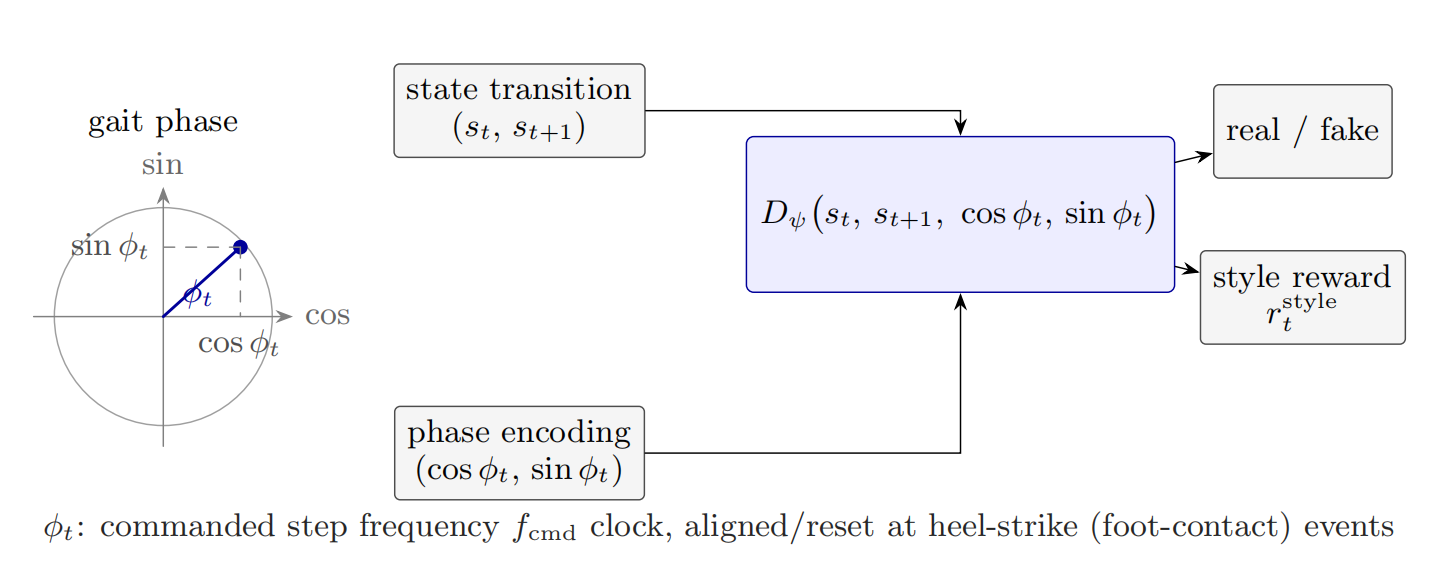
\includegraphics[width=\linewidth]{fig3.jpg}
  \caption{Phase-conditioned discriminator (contribution 2). A gait phase $\phi_t$ driven by foot-contact events is encoded as $(\cos\phi_t,\sin\phi_t)$ and concatenated to the discriminator input, so the discriminator learns phase-consistent style and suppresses within-cycle fluctuation.}
  \label{fig:phase}
\end{figure}

\subsection{Stability-Driven Adaptive Style-Weight Curriculum}
\label{subsec:method_curriculum}

A fixed $w^{\mathrm{style}}$ destabilizes early training when high and yields stiff gaits when low. We modulate style intensity via a slow moving average of the gate:
\begin{equation}
\bar g_t = \alpha\,g(m_t) + (1-\alpha)\,\bar g_{t-1},\qquad
\lambda_t = \lambda_{\max}\cdot \bar g_t,
\label{eq:ema}
\end{equation}
with $\alpha=0.01$ and $\lambda_{\max}=0.5$. The unified objective is
\begin{equation}
r_t = r^{\mathrm{task}}_t + \lambda_t \cdot r^{\mathrm{style}}_t = r^{\mathrm{task}}_t + \lambda_{\max}\,\bar{g}_t \cdot g(m_t)\,r^{\mathrm{amp}}_t.
\label{eq:total}
\end{equation}
This gives a dual-timescale mechanism: the fast gate $g(m_t)$ provides step-level safety interlocks, while the slow curriculum $\lambda_t$ schedules imitation difficulty across training.

% Declared before the Experiments section so this full-width float is placed at
% the top of the experiments page instead of being deferred into the references
% (it is referenced in Sec.~\ref{subsec:results}).
\begin{table*}[t]
  \centering
  \caption{Benchmarking and ablation across simulated protocols (5 random seeds; mean $\pm$ std.\ in MuJoCo). All methods achieve 100\% survival under nominal flat walking. Planar touchdown is the stance percentage free of ankle inversion/eversion tilting.}
  \label{tab:comparison}
  \small
  \begin{tabular}{lcccc}
    \toprule
    Configuration / Method & Push$\times3$ Survival & Rough Survival & Spectral Energy $\downarrow$ ($10^{-3}$) & Planar Touchdown $\uparrow$ \\
    \midrule
    \multicolumn{5}{l}{\textit{\textbf{Baseline Comparisons}}} \\
    Pure RL & $0.435 \pm 0.038$ & $0.245 \pm 0.032$ & $4.52 \pm 0.28$ & $54.2\% \pm 3.6\%$ \\
    Standard AMP & $0.462 \pm 0.041$ & $0.218 \pm 0.035$ & $2.48 \pm 0.16$ & $46.8\% \pm 4.2\%$ \\
    \textbf{SG-AMP (Ours)} & $\mathbf{0.736 \pm 0.032}$ & $\mathbf{0.386 \pm 0.035}$ & $\mathbf{1.65 \pm 0.12}$ & $\mathbf{85.4\% \pm 2.1\%}$ \\
    \midrule
    \multicolumn{5}{l}{\textit{\textbf{Ablation Configurations}}} \\
    SG-AMP $-$ G1 (w/o CoP Gate) & $0.512 \pm 0.036$ & $0.258 \pm 0.034$ & $1.92 \pm 0.14$ & $49.6\% \pm 3.9\%$ \\
    SG-AMP $-$ G2 (w/o Phase Disc.) & $0.648 \pm 0.035$ & $0.334 \pm 0.038$ & $3.08 \pm 0.21$ & $81.2\% \pm 2.6\%$ \\
    SG-AMP $-$ G3 (w/o Dynamic $\lambda_t$) & $0.615 \pm 0.042$ & $0.305 \pm 0.039$ & $1.85 \pm 0.15$ & $76.8\% \pm 3.2\%$ \\
    \bottomrule
  \end{tabular}
\end{table*}

\subsection{Training Procedure}
\label{subsec:method_training}

Fig.~\ref{fig:overview} and Algorithm~\ref{alg:sgamp} summarize SG-AMP.

\begin{algorithm}[t]
  \caption{SG-AMP training (PPO, simulation only).}
  \label{alg:sgamp}
  \begin{center}
  \small
  \renewcommand{\arraystretch}{1.1}
  \begin{tabular}{@{}r@{\hspace{0.9em}}l@{}}
    1: & Initialize $\pi_\theta$, $D_\psi$; $\phi_0{=}0$, $\bar g_0{=}0$; load reference $\mathcal{M}$. \\
    2: & \textbf{for} iteration $=1,2,\dots$ \textbf{do} \\
    3: & \quad \textbf{for} each environment and time step $t$ \textbf{do} \\
    4: & \quad\quad Read contact forces $f_{z,i}$ and foot poses; compute \\
       & \quad\quad\quad $p_{\mathrm{CoP}}$ and support polygon; \\
       & \quad\quad\quad margin $m_t$, gate $g(m_t)$. \hfill [G1] \\
    5: & \quad\quad Update phase $\phi_t$; compute $r^{\mathrm{task}}_t$. \hfill [G2] \\
    6: & \quad\quad $r^{\mathrm{style}}_t = g(m_t)\,\max\big(0,\,1-\tfrac14\,(D_\psi-1)^2\big)$, \\
       & \quad\quad\quad with $D_\psi = D_\psi(s_t,s_{t+1},\cos\phi_t,\sin\phi_t)$. \\
    7: & \quad\quad $\bar g_t = \alpha\,g(m_t)+(1-\alpha)\,\bar g_{t-1}$; \hfill [G3] \\
       & \quad\quad $r_t = r^{\mathrm{task}}_t + \lambda_{\max}\,\bar g_t\,r^{\mathrm{style}}_t$. \\
    8: & \quad \textbf{end for} \\
    9: & Update $D_\psi$ on $(\mathcal{M},\text{rollouts})$ under phase conditioning; \\
       & update $\pi_\theta$ with PPO. \\
    10: & \textbf{end for} \\
  \end{tabular}
  \end{center}
\end{algorithm}

\noindent\textbf{Implementation notes.}
An Isaac Lab parallel-RL template (Isaac Sim PhysX, $\sim$4096 environments, PPO) hosts the self-developed biped URDF. Per-foot net contact forces come from PhysX contact sensors (MuJoCo in sim2sim); because PhysX exposes no per-contact-point positions, each foot sole is reconstructed as a rectangle (four corners) whose convex hull is the support polygon. Reference data are retargeted MoCap, or privileged-expert trajectories as a fallback (Sec.~\ref{subsec:setup}). The phase uses a commanded-frequency clock with heel-strike alignment.

\section{Experiments}
\label{sec:experiments}

\subsection{Experimental Setup}
\label{subsec:setup}

\textbf{Robot and simulation.} Self-developed biped: $1.75$\,m tall, $60.9$\,kg, floating base, $12$ actuated revolute joints ($6$/leg: hip pitch/roll/yaw, knee pitch, ankle pitch/roll) and unactuated arms; thigh/shank $0.363$/$0.374$\,m; each $0.27\times0.10$\,m foot sole carries a $3\times2$ grid of six box contact bodies supplying the CoP-gate contact geometry. Actuation is joint-level PD at $50$\,Hz ($0.005$\,s step). Training in Isaac Sim (PhysX) \cite{mittal2023isaaclab} with GPU-parallel environments \cite{makoviychuk2021isaacgym}; zero-shot evaluation in MuJoCo \cite{todorov2012mujoco}.

\textbf{Reference data.} Public MoCap retargeted to the robot; fallback: privileged-expert trajectories per terrain (as in T-GMP \cite{guo2026tgmp}).

\textbf{Protocols.} Train on flat terrain with randomly sampled velocity commands; zero-shot evaluation covers (1) flat tracking, (2) external pushes (strength $\times3$), and (3) out-of-domain rough terrain (sim-to-sim generalization).

\subsection{Baselines, Metrics, and Ablations}

Baselines: \emph{Pure RL} (task reward only), \emph{AMP} \cite{peng2021amp} (fixed $w^{\mathrm{style}}$), and \emph{SG-AMP} (ours). Metrics (all simulation-computable): survival rate; spectral energy (jitter); style-reward variance (phase consistency); CoP margin statistics; and planar-touchdown ratio (stance free of ankle inversion/eversion). Ablations remove one module each: \emph{SG-AMP $-$G1} ($g\equiv1$), \emph{$-$G2} (no phase input), \emph{$-$G3} ($\lambda_t\equiv\lambda_{\max}$).

\subsection{Results}
\label{subsec:results}

All policies are evaluated over 5 random seeds with zero-shot transfer in MuJoCo. Under nominal flat walking every method achieves $100\%$ survival, so flat survival is omitted as non-discriminative. Table~\ref{tab:comparison} reports push and rough-terrain robustness plus spectral energy and planar touchdown.

\paragraph{Gait kinematics and contact stability}
As shown in the walking snapshots (Fig.~\ref{fig:snapshots}), SG-AMP produces a fluid, anthropomorphic gait with upright torso and natural swing clearance, avoiding the excessive knee flexion of Pure RL. In the MuJoCo contact analysis (Fig.~\ref{fig:grf}), standard AMP and Pure RL suffer ankle tilting at touchdown, yielding low planar-touchdown ratios ($46.8\%$/$54.2\%$) and localized impact forces that degrade push recovery ($0.462$) and rough-terrain traversal ($0.218$). SG-AMP enforces planar foot alignment ($85.4\%$), lifting push survival by $+59.3\%$ and rough survival by $+122.9\%$ over AMP.

\begin{figure}[H]
  \centering
  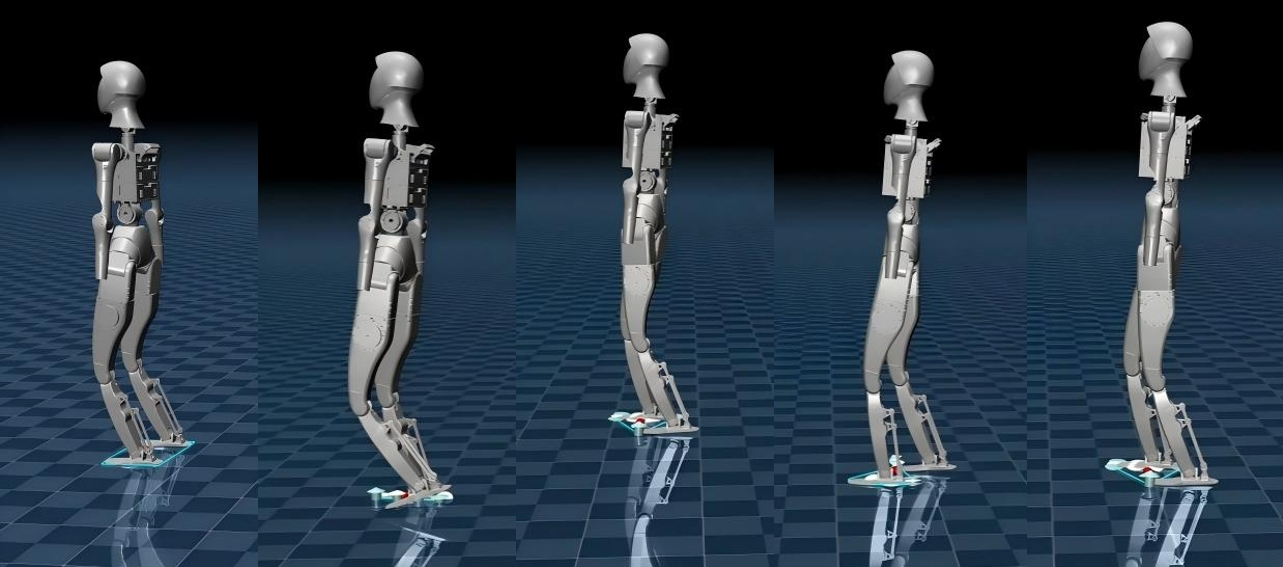
\includegraphics[width=\linewidth]{fig7.jpg}
  \caption{Consecutive walking snapshots of the SG-AMP policy in simulation, showing a stable, upright bipedal gait.}
  \label{fig:snapshots}
\end{figure}

\begin{figure}[H]
  \centering
  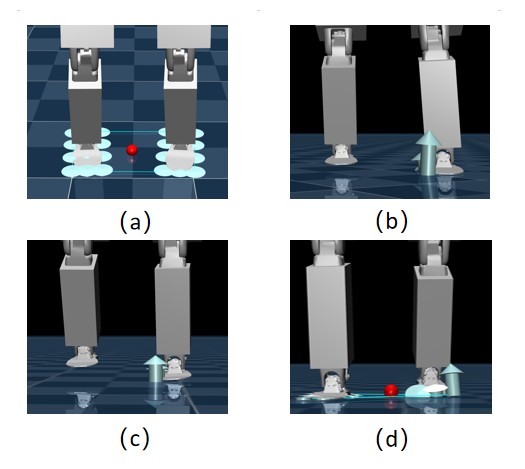
\includegraphics[width=0.78\linewidth]{fig8.png}
  \caption{Foot-ground interaction and ground-reaction-force (GRF) analysis in MuJoCo. (a) Each foot is modeled with multiple contact points to evaluate support geometry. (b) Standard AMP and (c) vanilla PPO exhibit severe foot tilt at touchdown (edge contact); (d) SG-AMP enforces planar alignment and a more uniform GRF distribution.}
  \label{fig:grf}
\end{figure}

\paragraph{Ablation study}
The lower partition of Table~\ref{tab:comparison} validates each component. Removing the CoP gate ($-$G1) drops push survival to $0.512$ and planar touchdown to $49.6\%$, since unconstrained style rewards encourage unstable edge landing---the core value of contribution 1. Removing phase conditioning ($-$G2) inflates spectral energy from $1.65$ to $3.08\times10^{-3}$ ($+86.7\%$), confirming that phase conditioning suppresses within-cycle discriminator noise and joint flutter. Fixing $\lambda_t\equiv\lambda_{\max}$ ($-$G3) degrades rough-terrain survival to $0.352$, showing the curriculum avoids adversarial conflict during early stabilization.

\paragraph{Gate behavior under stress}
The adaptive gate acts as intended: in steady flat walking the margin stays positive (minimum $+0.0086$\,m) and the gate engages only $8.4\%$ of stance ($g<0.8$); under severe pushes and irregular terrain the minimum margin turns negative and the gate activates for $35.6\%$/$44.2\%$ of stance, suppressing style until stability is regained.

\section{Conclusion}
\label{sec:conclusion}

We presented SG-AMP, which addresses three limitations of vanilla AMP---a physics-blind style reward, a phase-agnostic discriminator, and a fixed task--style weight---with three lightweight, independently ablating modules: a CoP-gated style reward, a phase-conditioned discriminator, and an adaptive style-weight curriculum. Requiring only foot contact forces and foot-sole geometry, SG-AMP suppresses joint flutter, eliminates edge landing, and improves push and rough-terrain robustness in simulation. Future work includes zero-shot hardware transfer and perceptive multi-terrain extension.

\section*{Acknowledgment}
This work was supported in part by the National Natural Science Foundation of China under Grants 92367109, 61973035, and 61803034; in part by the Beijing Natural Science Foundation under Grant L247007; in part by the R\&D Program of Beijing Municipal Education Commission under Grant KM202411417006; and in part by the Beijing Union University High-level Fund Incubation Project under Grant ZK20202509.

\bibliographystyle{unsrt}
\bibliography{refs}

\end{document}
